\newcommand{\nom}{Porte conteneur}
\newcommand{\sequence}{03}
\newcommand{\num}{04}
\newcommand{\type}{TD}
\newcommand{\descrip}{Résolution d'un problème en utilisant des méthodes algorithmiques}
\newcommand{\competences}{Alt-C3: Concevoir un algorithme répondant à un problème précisément posé}
\documentclass[10pt,a4paper]{article}
  \usepackage[french]{babel}
  \usepackage[utf8]{inputenc}
  \usepackage[T1]{fontenc}
  \usepackage{xcolor}
  \usepackage[]{graphicx}
  \usepackage{makeidx}
  \usepackage{textcomp}
  \usepackage{amsmath}
  \usepackage{amssymb}
  \usepackage{stmaryrd}
  \usepackage{fancyhdr}
  \usepackage{lettrine}
  \usepackage{calc}
  \usepackage{boxedminipage}
  \usepackage[french,onelanguage, boxruled,linesnumbered]{algorithm2e}
  \usepackage[colorlinks=false,pdftex]{hyperref}
  \usepackage{minted}
  \usepackage{url}
  \usepackage[locale=FR]{siunitx}
  \usepackage{multicol}
  \usepackage{tikz}
  \makeindex

  %\graphicspath{{../Images/}}

%  \renewcommand\listingscaption{Programme}

  %\renewcommand{\thechapter}{\Alph{chapter}}
  \renewcommand{\thesection}{\Roman{section}}
  %\newcommand{\inter}{\vspace{0.5cm}%
  %\noindent }
  %\newcommand{\unite}{\ \textrm}
  \newcommand{\ud}{\mathrm{d}}
  \newcommand{\vect}{\overrightarrow}
  %\newcommand{\ch}{\mathrm{ch}} % cosinus hyperbolique
  %\newcommand{\sh}{\mathrm{sh}} % sinus hyperbolique

  \textwidth 160mm
  \textheight 250mm
  \hoffset=-1.70cm
  \voffset=-1.5cm
  \parindent=0cm

  \pagestyle{fancy}
  \fancyhead[L]{\bfseries {\large PTSI -- Dorian}}
  \fancyhead[C]{\bfseries{{\type} \no \numero}}
  \fancyhead[R]{\bfseries{\large Informatique}}
  \fancyfoot[C]{\thepage}
  \fancyfoot[L]{\footnotesize R. Costadoat, C. Darreye}
  \fancyfoot[R]{\small \today}
  
  \definecolor{bg}{rgb}{0.9,0.9,0.9}
  
  
  % macro Juliette
  
\usepackage{comment}   
\usepackage{amsthm}  
\theoremstyle{definition}
\newtheorem{exercice}{Exercice}
\newtheorem*{rappel}{Rappel}
\newtheorem*{remark}{Remarque}
\newtheorem*{defn}{Définition}
\newtheorem*{ppe}{Propriété}
\newtheorem{solution}{Solution}

\newcounter{num_quest} \setcounter{num_quest}{0}
\newcounter{num_rep} \setcounter{num_rep}{0}
\newcounter{num_cor} \setcounter{num_cor}{0}

\newcommand{\question}[1]{\refstepcounter{num_quest}\par
~\ \\ \parbox[t][][t]{0.15\linewidth}{\textbf{Question \arabic{num_quest}}}\parbox[t][][t]{0.85\linewidth}{#1\label{q\the\value{num_quest}}}\par
~\ \\}

\newcommand{\reponse}[4][1]
{\noindent
\rule{\linewidth}{.5pt}\\
\textbf{Question\ifthenelse{#1>1}{s}{} \multido{}{#1}{%
\refstepcounter{num_rep}\ref{q\the\value{num_rep}} }:} ~\ \\
\ifdef{\public}{#3 ~\ \\ \feuilleDR{#2}}{#4}
}

\newcommand{\cor}
{\refstepcounter{num_cor}
\noindent
\rule{\linewidth}{.5pt}
\textbf{Question \arabic{num_cor}:} \\
}


%\usepackage{enumitem}

%\setenumerate[1]{align=left,label=\arabic*}
%\setenumerate[2]{before=\stepcounter{enumi},label*=.\arabic*,leftmargin=1.2em,align=left}

\usepackage{variations} 

\ifdef{\public}{\excludecomment{solution}}


\begin{document}

\begin{center}
{\Large\bf {\type} \no {\numero}}
\end{center}

\SetKw{KwFrom}{de} 

\begin{boxedminipage}{.9\textwidth} 
\begin{itemize}
 \item Faire tous les exercices dans un même fichier {NomPrenom.py} à sauvegarder,
 \item mettre en commentaire l'exercice et la question traités (ex: \# Exercice 1),
 \item ne pas oublier pas de commenter ce qui est fait dans votre code (ex: \# Je crée une fonction pour calculer la racine d'un nombre),
 \item il est possible de demander un déblocage pour une question mais uniquement celles avec une $\star$. Celle-ci sera notée 0,
 \item il faut vérifier avant de partir que le code peut s'exécuter et qu'il affiche les résultats que vous attendez.
\end{itemize}
\end{boxedminipage}




\section*{Exercice 1}
Pour tout entier naturel $n$, on considère la fonction $f_n$ définie sur $\mathbb{R} $ par : 
\[f_n(x) = x^{n+1}-x^n- 1.\]
On admet les résultats suivants sur $f_n$ : 
\begin{itemize}
\item[$\centerdot$] le tableau de variations de $f_n$ est : 
\begin{center}
\begin{variations}
x	   &	\; 1\;	 &\quad & \alpha_n & \quad &   	\pI  \\ \filet
\m{f_n}	    &	\; -1\;	 &\cb & \m{\;0\;} & \ch &    	\h \pI \\ \filet
\end{variations}
\end{center}
\item[$\centerdot$] $f_n(2)>0$ pour $n\geq 1$.
\end{itemize}\medskip 
Donc il existe un unique $\alpha_n\in[1,2]$ tel que $f_n$ s'annule en $\alpha_n$. L'objectif est d'étudier la suite $(\alpha_n)_{n\in\mathbb{N}}$. \medskip 
\begin{enumerate}
%\item Au brouillon, étudier les variations de $f_n$. Montrer notamment que $f_n$ est strictement croissante sur $[1,+\infty [$ et que $f_n(2) > 0$ si $n \geq  1$.
%\item  On note $\alpha_n$ l'unique solution de $f_n(x) = 0$ sur $[1, 2]$. Que vaut $\alpha_0$ ?
\item $\!\star$ Soit $n$ fixé en amont. Ecrire une fonction \verb?f? qui prend comme argument $x$ et renvoie la valeur de $f_n(x)$.
\item Afficher la valeur de $f_{10}(1)$.
\item Tracer les courbes de $f_n$, pour $n$ entier de $1$ à $10$. La plage d'affichage sera le rectangle $[1, 2]\times [-1, 1]$ (fonctions \texttt{xlim} et \texttt{ylim} du module \texttt{matplotlib.pyplot} en \textit{Python}). 
\item Conjecturer le comportement de la suite $(\alpha_n)_{n\geq  0}$ : monotonie, limite (réponse en commentaire).
%\end{enumerate}
%On rappelle ci-dessous l'algorithme de dichotomie.\\
%Soit $f$ continue sur un segment $[a, b]$ à valeurs réelles. On suppose que $f$ s'annule exactement une fois sur
%$[a, b]$ en un point que l'on note $\alpha$. On définit les suites $(a_k)_{k\geq  0}$ et $(b_k)_{k\geq  0}$ de la façon suivante :
%\begin{itemize}
%\item[$\centerdot$]  $a_0=a$ et $b_0=b$.
%\item[$\centerdot$]  On pose : $\forall k\in \mathbb{N},~~ c_k = \dfrac{a_k + b_k}{2}$ et 
%\begin{align*}
%\text{si } f(a_k)f(c_k)\leq 0, & \text{ alors } a_{k+1}=a_k\text{ et }b_{k+1}=c_k,\\
%& \text{ sinon }a_{k+1}=c_k\text{ et }b_{k+1}=b_k.
%\end{align*}
%\end{itemize}
%On sait qu'alors les deux suites $(a_k)_{k \geq  0}$ et $(b_k)_{k\geq  0}$ convergent toutes les deux vers $\alpha$, en vérifiant :
%$$ \forall k\in \mathbb{N},~~ a_k \leq \alpha \leq b_k \text{ et } \forall k \in\mathbb{N},~~ b_k - a_k =
%\dfrac{b-a}{2^k} .$$
%On peut alors montrer que si $b_k - a_k\leq \varepsilon$, alors $a_k$ et $b_k$ sont des valeurs approchées de $\alpha$ à $\varepsilon$ près.
%\begin{enumerate}
%\setcounter{enumi}{4}
\item $\star$ Écrire une fonction \verb?dichotomie? qui prend comme entr\' ee une fonction $f$, les bornes initiales $a$ et $b$, la pr\' ecision $\varepsilon$ et qui renvoie une approximation d’une solution \` a $\varepsilon$ pr\` es de l'équation $f(x)=0$ de l'intervalle $[a,b]$.
\item En utilisant l'algorithme précédent, déterminer des valeurs approchées de $\alpha_n$ à $10^{-6}$ près pour $n$ variant de $2$ à $200$. Quelle conjecture pouvez-vous faire ? (réponse en commentaire).
%\item Pour ces mêmes valeurs de $n$, comparer $\alpha_n$ avec la formule empirique $(1 + 1.6 (n + 2.6)^{-0.83})$.
\end{enumerate}







\section*{Exercice 2}
\begin{enumerate}
\item Préliminaires :\\
Ecrire une fonction \verb?maxi? qui prend comme argument une liste et renvoie la valeur maximale ainsi que sa position dans la liste. Si il y a plusieurs maxima, la fonction ne renvoie que la première position.\\
\textit{Dans cette question l'utilisation des fonctions Python \verb?max? et \verb?index? sont interdites.}
\begin{minted}{python}
>>>L=[1,8,1,-2,-7,8]
>>>maxi(L)
(8,1)
\end{minted}
\end{enumerate}


\vfill {\Large\textbf{TOURNEZ LA PAGE.}}
\newpage


Dans cet exercice, on manipule des suites (finies) d'entiers sous la forme de listes d'entiers. Ainsi la suite $(0,1,3,8,8)$ sera représentée par la liste \texttt{[0,1,3,8,8]}.\\
La liste est croissante (respectivement décroissante, monotone) si la suite est croissante (respectivement décroissante, monotone). 
\begin{enumerate}
\setcounter{enumi}{1}
\item Monotonie :
\begin{enumerate}
\item Ecrire une fonction \texttt{estCroissante} qui teste si une liste d'entiers est croissante. La fonction renvoie un booléen \verb?True? ou \verb?False?. %Cette fonction devra être de complexité linéaire.
\item Afficher le résultat de la fonction \verb?estCroissante? pour la liste \verb?L=[0,1,3,8,8]?. (La réponse doit être \verb?True?).
\item \'Ecrire de même une fonction \texttt{estDecroissante} qui teste si une liste d'entiers est décroissante.
\item \'Ecrire de même une fonction \texttt{estMonotone} qui teste si une liste d'entiers est monotone.
\end{enumerate}
\item Soit la liste $L=[u_0,u_1,\cdots,u_{n-1}]$ de longueur $n$. On appelle tranche de $L$ une liste de la forme $[u_i,u_{i+1},\cdots,u_j]$ où $0\leq i \leq j <n$.\\
On cherche une tranche de $L$ croissante et de longueur maximale.\\
Par exemple, une tranche croissante de longueur maximale de $[0,1,0,1,3,3,5,0,1,7]$ est $[0,1,3,3,5]$, correspondant aux indices $i=2$ et $j=6$.
\begin{enumerate}
\item $\star$ \'Ecrire une fonction \texttt{LC} de deux arguments, une liste \texttt{L} et un entier \texttt{p}, qui renvoie l'entier \texttt{d} tel que la liste $\texttt{[u}_\texttt{p},\cdots,\texttt{u}_\texttt{d}\texttt{]}$ est la tranche croissante de $L$ la plus longue possible en partant de la $\texttt{p}$ième position. Autrement dit,  $\texttt{[u}_\texttt{p},\cdots,\texttt{u}_\texttt{d}\texttt{]}$ est croissante avec ou bien \texttt{d=n-1} ou bien $\texttt{u}_{\texttt{d}}>\texttt{u}_{\texttt{d+1}}$. 
\item Afficher le résultat de \texttt{LC} pour la liste \verb?L=[0,1,0,1,3,3,5,0,1,7]? et l'entier 2.
\item \'Ecrire une fonction \texttt{maxCroissante} d'argument une liste \texttt{L} qui renvoie la plus longue tranche croissante de \texttt{L}. S'il n'y a pas unicité, on renvoie la première trouvée.
\end{enumerate}
\item Soit la liste $L=[u_0,u_1,\cdots,u_{n-1}]$ de longueur $n$. Une monotonie de $L$ est un couple d'indices $(i,j)$ tel que $0\leq i < j < n$, que la sous-liste $[u_i,u_{i+1},\cdots,u_{j}]$ est monotone et qu'elle ne l'est plus si on l'étend, à droite ou à gauche, d'un élément supplémentaire (lorsque c'est possible). La monotonie est dite ``banale'' lorsque $j=i+1$.
\begin{enumerate}
\item Proposez une liste d'entiers de longueur $5$ qui ne présente que des monotonies banales. (réponse en commentaire)%Peut-on avoir deux termes consécutifs égaux dans une liste ne présentant que des monotonies banales ? (on mettra la réponse en commentaire)
\item \'Ecrire une fonction \texttt{cahots}, de complexité linéaire, qui teste si une liste ne comporte que des monotonies banales.
\item Après avoir créé une liste arbitraire \texttt{L} de valeurs toutes distinctes, on peut l'ordonner par \texttt{L.sort()}. Imaginer ensuite une méthode pour réordonner de manière à ce qu'elle ne comporte que des monotonies banales.
\end{enumerate}
\end{enumerate}


\end{document}














\section*{Exercice}
On définit les suites $(a_n)$ et $(b_n)$
par :
$$\begin{cases}a_0=u\\ b_0=v\end{cases} \text{ et, pour tout }n\in \mathbb{N},~~ \begin{cases}a_{n+1}=\sqrt{a_nb_n}\\ 
b_{n+1}=\frac{2}{\frac{1}{a_n}+\frac{1}{b_n}}\end{cases},$$
où $u$ et $v$ sont deux réels strictement positifs.
\begin{enumerate}
\item Écrire une fonction \texttt{iterer}  d'un seul argument $p$, où $p$ représente le couple 
$(a_n,b_n)$, et qui renvoie le couple $(a_{n+1},b_{n+1})$. Tester cette fonction en calculant \texttt{iterer([3,2])}.
\item Créer une fonction \textit{non récurive} \texttt{suite} de trois $u$, $v$ et $n$ et qui renvoie 
le couple $(a_n,b_n)$.
\item Tester cette fonction en calculant \texttt{suite(3,2,2)}, puis \texttt{suite(3,2,5)}; que peut-on conjecturer ?
\item On admet que pour deux réels strictement positifs donnés $u$ et $v$, les suites $(a_n)_{n\in \mathbb{N}}$ et $(b_n)_{n\in \mathbb{N}}$ convergent vers une même limite $\ell$  qu'elles encadrent (ie, pour $n\geq  1$,  $b_n\leq  \ell \leq a_n$). Créer une fonction \texttt{moyenne}  de deux arguments $u$ et $v$ qui renvoie  une valeur approchée à $10^{-10}$ près par défaut de cette limite. 
%\item Créer une fonction \textit{récursive} \texttt{suiterec} de trois arguments $u$, $v$ et $n$ qui renvoie le  couple $(a_n,b_n)$. Tester cette fonction par \texttt{suiterec(3,2,5)};
\item Faire tracer \texttt{moyenne(1,x)} pour $x$ variant entre $1$ et $10$ avec un pas de $0,1$.
\end{enumerate}







\end{document}

\section{Bof}


\begin{exercice}
\begin{enumerate}
\item \'Ecrire une fonction \texttt{binaire} d'argument un entier naturel $n$ et qui renvoie la liste des chiffres, bit de poids fort en tête, de l'écriture en base $2$ de $n$. Par exemple, \texttt{binaire(23)} renvoie \texttt{[1,0,1,1,1]}.
\item \'Ecrire une fonction \texttt{nombreDeUns} d'argument un entier naturel $n$, qui renvoie le nombre de chiffres de $1$ dans l'écriture binaire de $n$. Par exemple, \texttt{nombreDeUns(23)} renvoie $4$.
\item Soit $n$ un entier naturel. On dit que $n$ est un $2$-palindrome si sa représentation en base $2$ est la même, qu'elle soit écrite de gauche à droite ou de droite à gauche. Par exemple, $9$ est un $2$-palindrome car $9$ s'écrit $1001$ en base $2$.\\ \\
\'Ecrire une fonction \texttt{palindrome} d'argument un entier naturel $n$ qui renvoie un booléen indiquant si $n$ est un $2$-palindrome, ou pas.
\item Faire afficher tous les $2$-palindromes inférieurs à $100$.
\item \'Ecrire une fonction \texttt{baseB} de deux arguments, un entier naturel $n$ et un entier $b$ compris entre $2$ et $10$, qui renvoie la liste des chiffres, chiffre de poids fort en tête, de l'écriture en base $b$ de $n$.
\item Faire afficher les $10$ plus petits entiers naturels non nuls qui sont à la fois des $4$-palindromes et des $9$-palindromes.
\end{enumerate}
\end{exercice}



\begin{exercice}
L'objet de cet exercice est d'étudier numériquement la série $\sum \dfrac{(-1)^{n+1}}{n}$.
\begin{enumerate}
\item On admet que cette série est convergente et que $\left| \sum\limits_{k=n}^{+\infty}\frac{(-1)^{k+1}}{k}\right|<\frac{1}{n}$. \\
Donner une valeur approchée à $10^{-6}$ près de la somme de cette série. Vérifier que cette valeur est proche de \texttt{log(2)} où \texttt{log} désigne la fonction logarithme népérien. 
\item Représenter graphiquement les cent premières sommes partielles de cette série.
\item On modifie l'ordre des termes de la série en prenant alternativement $2$ termes positifs et $3$ termes négatifs comme suit :
$$\left(1+\frac{1}{3}\right)+\left(-\frac{1}{2}-\frac{1}{4}-\frac{1}{6}\right)+\left(\frac{1}{5}+\frac{1}{7}\right)+\left(-\frac{1}{8}-\frac{1}{10}-\frac{1}{12}\right)+\cdots$$
\'Ecrire une fonction \texttt{SDP} d'argument un entier naturel $n$ non nul et qui renvoie la liste des $n$ premières sommes partielles de cette série réordonnée.
\item Représenter graphiquement les $120$ premières valeurs de cette série réordonnée. Que peut-on conjecturer sur la somme de cette série ?
\item Examiner ce qui se passe si l'on prend un terme positif, puis un terme négatif, puis deux positifs, puis un seul négatif, puis trois positifs, puis un seul négatif, puis quatre positifs, etc.
\end{enumerate}
\end{exercice}




\begin{exercice}
\begin{enumerate}
\item Soit le système différentiel avec condition initial suivant :
\begin{equation}\label{eqn:systeme}
\begin{cases} x'(t)  =  y(t) \\
y'(t)  = (1-x(t)^2)y(t)-x(t) \\
x(0) =  2 \\
y(0) =  0 \end{cases}
\end{equation}
Pour un pas de discrétisation $h=\frac{1}{4}$, puis $h=\frac{1}{8}$, représenter, en fonction du temps, les solutions approchées de cette équation obtenues par la méthode d'Euler, pour $t$ dans l'intervalle $[0,8]$.
\item En utilisant la fonction \texttt{odeint} du module \texttt{scipy.integrate} de \textit{Python}, résoudre numériquement le problème (\ref{eqn:systeme}). On prendra garde à définir soigneusement les arguments de cette fonction en lisant attentivement l'aide en ligne.\\ \\
Représenter sur la figure précédente la solution numérique trouvée. 
\item Représenter les différentes solutions trouvées dans le plan $xy$. 
\item Représenter sur l'intervalle $[0,8]$ une solution approchée de l'équation $x''(t)=(1-x(t)^2)x'(t)-x(t)$ avec $x(0)=0$ et $x'(0)=1$.
\end{enumerate}
\end{exercice}




\begin{exercice} 
\begin{enumerate}
\item Soit $f$ la fonction définie sur $[-5,5]$ par $f(x)=\dfrac{1}{1+x^2}$. Tracer la courbe de $f$.\\ \\
\fbox{ \begin{minipage}{15cm}Il existe différentes méthodes pour approcher une fonction $h$ par un polynôme.\\
L'une d'entre elles, dite ``interpolation de Lagrange'', consiste à construire un polynôme de degré $(n-1)$ coïncidant en $n$ points avec la fonction $h$. \\
Plus précisément, si $h$ est définie sur un segment contenant les valeurs distinctes $[a_0,a_1,\cdots,a_{n-1}]$ regroupées dans une liste \textbf{a}, alors le polynôme :
$$P_{\text{\textbf{a}},h}(x)=\sum_{i=0}^{n-1}h(a_i)\left(\prod_{k=0,k\neq i}^{n-1}\frac{x-a_k}{a_i-a_k}  \right)$$
est le seul polynôme de degré inférieur ou égal à $(n-1)$ tel que 
$$\forall i\in \mathbb{N},~~0\leq i <n,~~P(a_i)=h(a_i).$$
\end{minipage}}
\item \'Ecrire une fonction \texttt{interpoler} de trois arguments, une fonction $h$, un réel $x$ et une liste \textbf{a} qui renvoie $P_{\text{\textbf{a}},h}(x)$.
\item \'Ecrire une fonction \texttt{affiche} d'argument $j$ donnant la représentation graphique de $f$ et de $P_{\text{\textbf{a}},f}$, $\textbf{a}$ correspondant aux $(j+1)$ valeurs équiréparties sur l'intervalle $[-5,5]$.
\item Tester la fonction précédente pour $j=5$, $10$, $15$, $20$. Qu'observe-t-on ?
\item Cette fonction particulière $f$ montre que l'interpolation par des points équirépartis n'est pas toujours adaptée pour obtenir une bonne approximation. Une façon de traiter ce problème consiste à ne plus faire l'interpolation de Lagrange sur des points équirépartis sur le segment, mais sur les abscisses dites ``de Thebychev'' :
$$a_i=5\cos\left( \frac{(2i+1)\pi}{2n}\right),~~i\in \mathbb{N},~~0\leq i <n.$$
Visualiser le résultat pour différentes valeurs de $n$.
\end{enumerate}
\end{exercice}






\begin{exercice}
On cherche à étudier numériquement les solutions de l'équation différentielle avec conditions initiales suivante 
\begin{equation}
y'(t)=t^2-y(t)^3~~\text{ avec }~~y(-1.5)=a. \label{eqn:equadiff23}
\end{equation}
\begin{enumerate}
\item Pour $a=2$ et un pas de discrétisation $h=\frac{1}{4}$, puis $h=\frac{1}{8}$, représenter les solutions approchées du problème (\ref{eqn:equadiff23}) obtenues par la méthode d'Euler sur l'intervalle $[-1.5,2.5]$.
\item En utilisant la fonction \texttt{odeint} du module \texttt{scipy.integrate} de \textit{Python}, résoudre numériquement le problème (\ref{eqn:equadiff23}) pour $a=2$. On prendra garde à bien définir soigneusement les arguments de cette fonction en lisant attentivement l'aide en ligne.
\item Sur la figure existante, rajouter la courbe de la solution numérique obtenue à la question précédente.
\item Rajouter ensuite les courbes des solutions  numériques pour $a=1.3$ et $a=0.1$. Qu'observe-t-on ?
\item Pour résoudre $y'(t)=f(t,y(t))$ avec $y(t_0)=a$, on utilise maintenant la suite $(y_n)$ définie par $y_0=a$ et $y_{k+1}=y_k+\dfrac{h}{2}\left( f(t_k,y_k)+f(t_{k+1},y_k+hf(t_k,y_k))\right)$. \\
Représenter, pour $a=2$ et les mêmes pas de discrétisation qu'à la question 1, les solutions approchées obtenues par cette méthode. Expliquer pourquoi le résultat semble meilleur.
\end{enumerate}
\end{exercice}


\begin{exercice}
Dans le plan affine, muni d'un repère orthonormé direct d'origine $O$, on considère la suite de point $(A_n)_{n\in \mathbb{N}}$ tels que :
\begin{itemize}
\item $A_0$ a pour coordonnées $(1,0)$.
\item pour tout entier naturel non nul $n$, le triangle $OA_nA_{n+1}$ est rectangle en $A_n$, la distance $A_nA_{n+1}$ vaut $1$ et l'angle $\left(\overrightarrow{OA_n},\overrightarrow{OA_{n+1}}\right)$ est direct.
\end{itemize}
\begin{multicols}{2}
Si $x_n$ et $y_n$ sont les coordonnées de $A_n$, on a :
$$\begin{cases} x_{n+1}=x_n-\dfrac{y_n}{\sqrt{x_n^2+y_n^2}}\\  \\ y_{n+1} = y_n+\dfrac{x_n}{\sqrt{x_n^2+y_n^2}}\end{cases}.$$
\\ 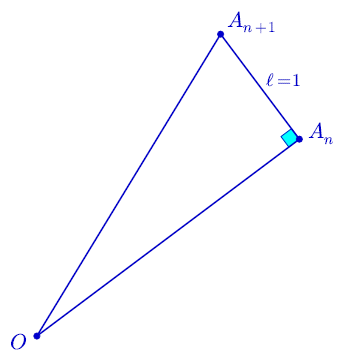
\includegraphics[scale=0.4]{ex24.png}
\end{multicols}
\begin{enumerate}
\item \'Ecrire une fonction \texttt{A} d'argument $N$ renvoyant la liste des coordonnées des points $A_n$ pour $0\leq n\leq N$. 
\item \'Ecrire une fonction \texttt{afficher} d'argument $N$ affichant la figure représentant les $(N+1)$ premiers points $A_n$. La tester pour $N=60$.
\end{enumerate}
Les points $A_k$ tournent autour de l'origine $O$ du repère. On note $T(k)$ la valeur de $n$ telle que le point $A_n$ commence le $k$-ième tour.
\begin{enumerate}
\setcounter{enumi}{2}
\item \'Ecrire une fonction \texttt{tours} d'argument $m$ qui renvoie la liste des $T(k)$ pour $k$ variant de $1$ à $m$. Afficher \texttt{tours(5)}.
\item Faire tracer chacun des cinq premiers tours avec une couleur différente.
\item Déterminer les abscisses des dix premiers points d'intersection de la ligne reliant les $A_n$ avec la partie positive de l'axe des abscisses. Vérifier qu'à chaque tour, on s'est éloigné du centre d'une distance environ égale à $\pi$.
\end{enumerate}
\end{exercice}





\begin{exercice}
Pour un entier naturel $n$ non nul fixé, on appelle \textit{vecteur creux} de $\mathbb{R} ^n$ un vecteur dont au moins la moitié des coefficients sont nuls. On code ces vecteurs à l'aide d'une liste de deux listes. La première est la liste des valeurs des coefficients non nuls, la seconde celle de leurs indices, rangés en ordre croissant.\\
Par exemple, le vecteur
$$v=\left( \begin{array}{cccccccccccc}
1 & 3 & 0 & 4 & 0 & 0 & 1 & 2 & 0 & 0 & 0 & 0
\end{array}\right)$$ est codé par : $$ [[1,3,4,1,2],[0,1,3,6,7]]$$
On a en effet $v_0=1$, $v_1=3$, $v_3=4$, $v_6=1$ et $v_7=2$. Les autres coefficients sont nuls.
\begin{enumerate}
\item \'Ecrire une fonction \texttt{creux} d'argument une liste simple représentant un vecteur $v$ qui renvoie un booléen indiquant si $v$ est creux ou pas.
\item \'Ecrire deux fonctions : \texttt{coder} d'argument un vecteur qui renvoie son codage ``creux''; \texttt{decoder} de deux arguments $C$ et $n$, qui restitue le vecteur de dimension $n$ à partir de son codage ``creux'' $C$.\\
\\
On construit maintenant des fonctions adaptées pour le codage ``creux''.
\item \'Ecrire une fonction \texttt{smul} de deux arguments $C$ et $a$, où $C$ est le codage ``creux'' d'un vecteur $v$ et $a$ un scalaire, qui renvoie le codage creux du vecteur $av$.
\item \'Ecrire une fonction \texttt{pscal} de deux arguments \texttt{C1} et \texttt{C2}, codages ``creux'' de deux vecteurs $v_1$ et $v_2$, qui renvoie le produit scalaire de ces deux vecteurs. 
\item \'Ecrire une fonction \texttt{add} de deux arguments \texttt{C1} et \texttt{C2}, codages ``creux'' de deux vecteurs $v_1$ et $v_2$, qui renvoie le codage ``creux'' du vecteur $v_1+v_2$. Cette somme est-elle toujours un vecteur creux ?
\end{enumerate}
\end{exercice}




\begin{exercice}
Une matrice carrée d'ordre $n$ est dite ``magique'' si elle contient tous les nombres de $1$ à $n^2$ et si les sommes des nombres de chaque ligne, de chaque colonne  et de chaque diagonale sont toutes  égales à une constante $s$.
\begin{enumerate}
\item Au brouillon, exprimer la constante $s$ en fonction de $n$.
\item Créer une fonction \texttt{EstMagique}, d'argument une matrice $T$ (carrée de taille $n$) et qui renvoie un booléen indiquant si $T$ est magique ou pas. \\
Tester cette fonction sur les matrices :
$$ A=\left(\begin{array}{ccc}
4 & 9 & 2 \\ 3 & 5 & 7 \\ 8 & 1 & 6
\end{array}\right)~~\text{ et }~~B=\left(\begin{array}{ccc}
1 & 8 & 2 \\ 4 & 5 & 7 \\ 6 & 9 & 3
\end{array}\right)$$
\end{enumerate}
Une méthode permettant de construire une matrice magique de taille impaire $n=2p+1$ est la suivante :
\begin{itemize}
\item On construit une matrice de taille $n$ remplie de zéros. On considère cette matrice comme la représentation sur une période d'une matrice infinie $n$-périodique en lignes et en colonnes.
\item On remplace ensuite les zéros de la matrice avec les nombres de $1$ à $n^2$ comme  suit :
\begin{itemize}
\item on met le $1$ dans la case située sous la case centrale de la matrice;
\item on place ensuite chaque nombre de $2$ à $n^2$ dans la case située ligne suivante et colonne suivante de celles où on a mis le nombre précédent. Si cette case est déjà remplie, on avance encore d'une ligne et on recule d'une colonne.
\end{itemize}
\end{itemize}
On admet que la matrice ainsi construite est magique.
\begin{enumerate}
\setcounter{enumi}{2}
\item Construire ``à la main'', selon cette méthode, une matrice magique d'ordre $3$.
\item \'Ecrire une fonction \texttt{Magique} d'argument un entier $p$ qui renvoie la matrice magique de taille $2p+1$ créée à l'aide de la méthode précédente.
\end{enumerate}
\end{exercice}





\end{document}
